\documentclass[a4paper,10pt]{article}
\usepackage[a4paper, total={6in, 8in}]{geometry}
\setlength\parindent{0pt}
\usepackage[utf8]{inputenc}
\usepackage{graphicx} 
\usepackage{amsmath}
\usepackage{amsfonts}
\usepackage{amssymb}
\usepackage{listings}
\usepackage{ragged2e}
\usepackage{listings}
\usepackage{color}
\usepackage{array}
\usepackage{soul}
\newcolumntype{P}[1]{>{\centering\arraybackslash}p{#1}}

\setlength{\parskip}{\baselineskip}%
\setlength{\parindent}{0pt}%

\begin{document}
\begin{titlepage}
	\centering
	
\includegraphics[width=.6\textwidth]{liu-logo.png}\par
	\vfill
	{\scshape\Large TDDE01 MACHINE LEARNING\par}
	{\huge\bfseries Lab 2 - Report\par}
	\vspace{0.5cm}
	{\large\itshape Lawrence Thanakumar Rajappa (lawra776)\par}
	\vfill
	{\large \today\par}
\end{titlepage}
\definecolor{dkgreen}{rgb}{0,0.6,0}
\definecolor{gray}{rgb}{0.5,0.5,0.5}
\definecolor{mauve}{rgb}{0.58,0,0.82}

\lstset{frame=tb,
  language=R,
  aboveskip=3mm,
  belowskip=3mm,
  showstringspaces=false,
  columns=flexible,
  basicstyle={\small\ttfamily},
  numbers=none,
  numberstyle=\tiny\color{gray},
  keywordstyle=\color{blue},
  commentstyle=\color{dkgreen},
  stringstyle=\color{mauve},
  breaklines=true,
  breakatwhitespace=true,
  tabsize=3
}

\textbf{\underline{Assignment - 1}} \par
1. Scatterplot of carapace length (CL) versus rear width (RW) 
\begin{center}
	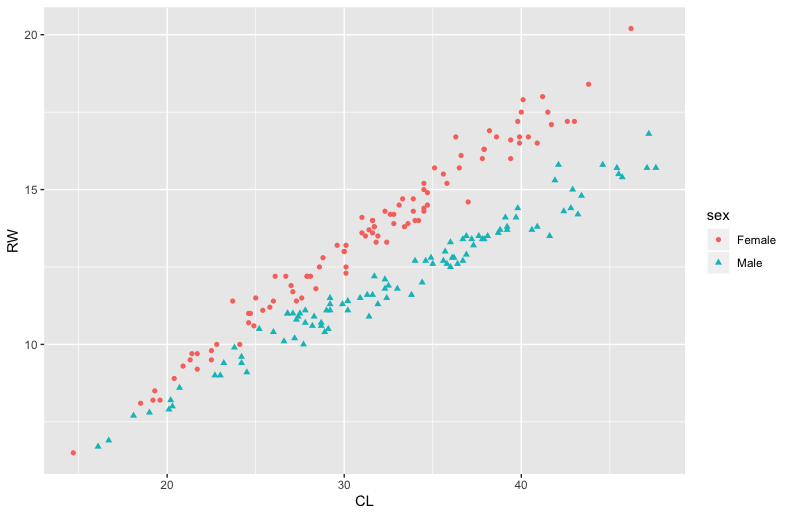
\includegraphics[width=125mm,scale=0.10]{CL_RW_Plot.png} 
\end{center} \par
The above plot describes the variables carapace length, rear width categorized by sex. From the plot we can observe
that, these two variables are not linearly separable and they overlap at the beginning of the plot.
Hence the \textit{\textbf{'species'}} cannot be a classified by other linear machine learning algorithms. We can use
Linear Discriminant Analysis (LDA) which focuses on maximizing the separability between two categories by, \par
\begin{center}
    \begin{itemize}
        \item \textbf{Maximizing the distance between two means (two categories)}
        \item \textbf{Minimizing the variation (scatter) in two categories}
    \end{itemize} \par
\end{center}
We can also use Principal Component Analysis (PCA), but the separation is not accurate when compared with LDA. \par
\vspace{0.5cm}
2. We have performed LDA on the \textit{\textbf{australian crabs}} dataset using \textit{lda()} in R. The target variable
sex and independent variables are caraspace length (CL) and rear width (RW) and obtained the following plot.
\begin{center}
  \includegraphics[width=125mm,scale=0.10]{CL_RW_Lda_Plot_1.png} \par
  \begin{tabular}{|c|}
		\hline
    \textbf{Confusion Matrix} \\
    \hline
    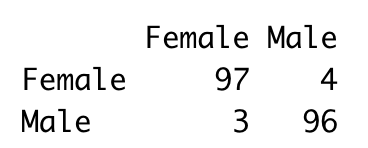
\includegraphics[width=50mm,scale=0.10]{CL_RW_LDA_Confusion_Matrix_1.png} \\
    \hline
  \end{tabular}\par
  \begin{tabular}{|c|}
    \hline
    \textbf{Missclassification Rate} \\
    \hline
    0.035 $\sim$ 3.5\% \\
    \hline
  \end{tabular}
\end{center} \par
I have compared the above plot with another plot from step 1 and found no difference and plots looks the same. By
looking at the confusion matrix and misclassification rate, I could see that LDA did a good job in classifying the 
data with minimal classification error i.e. 3.5\%. \par
\vspace{0.5cm}
3. By using prior probabilities, p(male) = 0.9 and p(female) = 0.1 generated the below plot with confusion matrix and
misclassification rates.
\begin{center}
  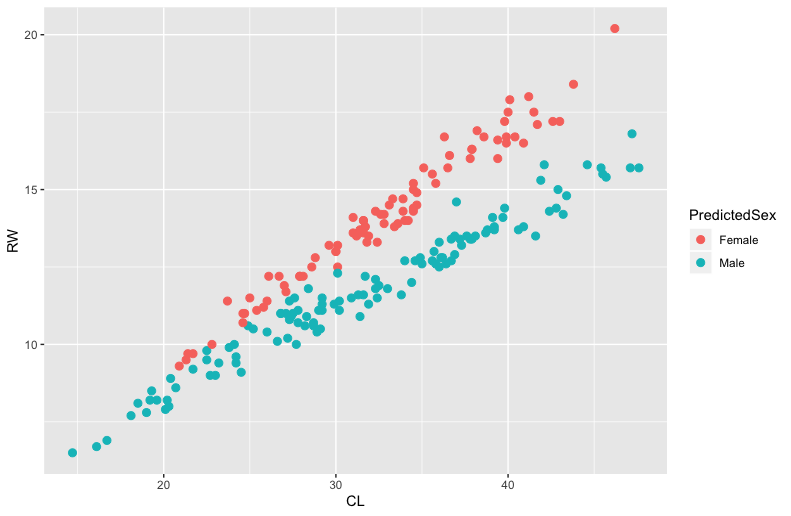
\includegraphics[width=125mm,scale=0.10]{CL_RW_Lda_Plot_Priors.png} 
  \begin{tabular}{|c|}
    \hline
    \textbf{Confusion Matrix} \\
    \hline
    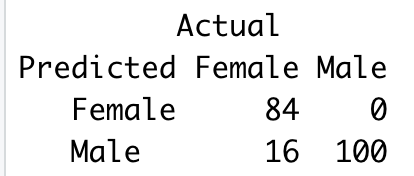
\includegraphics[width=50mm,scale=0.10]{CL_RW_LDA_Confusion_Matrix_Prior.png} \\
    \hline
  \end{tabular} \par
  \begin{tabular}{|c|}
    \hline
    \textbf{Missclassification Rate} \\
    \hline
    0.08 $\sim$ 8\% \\
    \hline
  \end{tabular}
\end{center} \par
From observing confusion matrix, plot and misclassification rate, I could say that LDA has classified most of the data as
\textbf{\textit{"Male"}} than female because in \textbf{step 1} we have given prior probabilitiy as 0.5 for each
category, but in this step, we have given higher probabilitiy to \textbf{\textit{"Male"}} than \textbf{\textit{"Female"}}. 
Based on the definition of Prior probability, it is like initial beliefs about an event. 
so when the algorithm sees the data it will classify the data based on the belief. Hence, according to confusion matrix,
total 100 data which was actually classified as \textbf{\textit{"Male"}} is predicted correctly, but 16 data which
were actually \textbf{\textit{"Female"}} but classified as \textbf{\textit{"Male"}}.\par
\vspace{0.5cm}
4. The given data was tested on Logistic regression with the default threshold value of \textbf{0.5} and have received
the below confusion matrix, misclassification rate and plot with decision boundary. \par
The decision boundary equation is,
    \begin{align*}
      \textbf{Slope} = \frac{\text{coef(Logistic Model)[2]}}{\text{-coef(Logistic Model)[3]}} = \frac{\text{4.630747}}{-(\text{-12.56389})} = 0.3685758 \\
      \textbf{Intercept} = \frac{\text{coef(Logistic Model)[1]}}{\text{-coef(Logistic Model)[3]}} = \frac{\text{13.61663}}{-(\text{-12.56389})} = 1.083791\\
      \textbf{Final Equation} = Slope*x+Intercept = 0.3685758*x+1.083791
    \end{align*}
  \begin{center}
    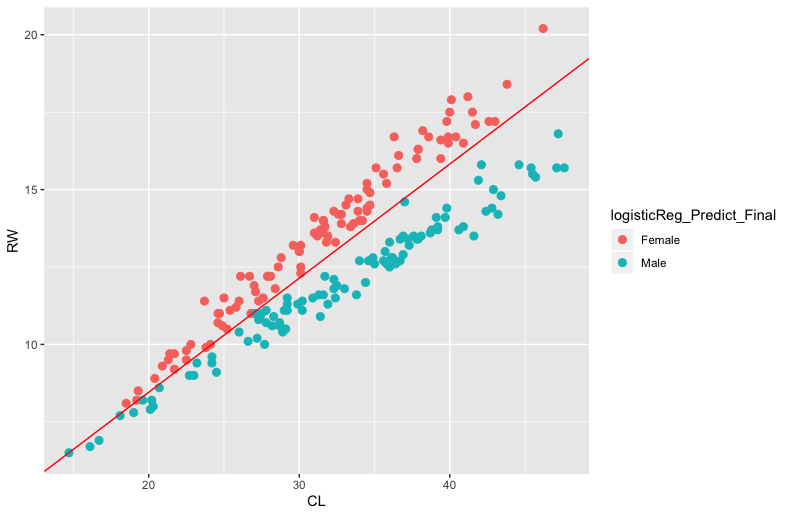
\includegraphics[width=125mm,scale=0.10]{CL_RW_Logistic_Regression_Plot.png} 
    \begin{tabular}{|c|}
      \hline
      \textbf{Confusion Matrix} \\
      \hline
      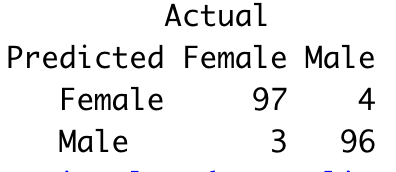
\includegraphics[width=50mm,scale=0.10]{CL_RW_Logistic_Regression_CM.png} \\
      \hline
    \end{tabular} \par
    \begin{tabular}{|c|}
      \hline
      \textbf{Missclassification Rate} \\
      \hline
      0.035 $\sim$ 3.5\% \\
      \hline
    \end{tabular}
  \end{center}
  From the confusion matrix and misclassification rate, I could see that the results are 
  same as the results in \textbf{step 2}. From this I can conclude that both LDA and Logistic regression works the same i.e. used for classification.
  But, differ in estimating the parameters i.e. LDA maximizes \textbf{complete likelihood} while Logistic Regression maximizes \textbf{conditional likelihood} only. \par
\newpage
\textbf{\underline{Assignment - 2}} \par
2. \textbf{\textit{\underline{Deviance and Gini Index}}} \par
\vspace{0.5cm}
\textbf{\textit{\underline{Misclassification Rates}}}
\begin{center}
  \begin{tabular}{|c|c|c|}
    \hline
    & Misclassification rate train & Misclassification rate test\\
    \hline
    Deviance &0.212 $\sim$ 21.2\% & 0.268 $\sim$ 26.8\% \\
    \hline
    Gini Index &0.24 $\sim$ 24\% & 0.368 $\sim$ 36.8\%\\
    \hline
  \end{tabular}
\end{center}\par
\vspace{0.5cm}
By comparing measures of impurity's misclassification rates, I have chosen \textbf{\textit{Deviance}}
as the measure of impurity which can be used to split the nodes because it has less misclassification 
rates than Gini index's misclassification rates.
\par
3. The below plot describes the dependance of deviance for the training and validation data on the number of leaves. \par
\begin{center}
  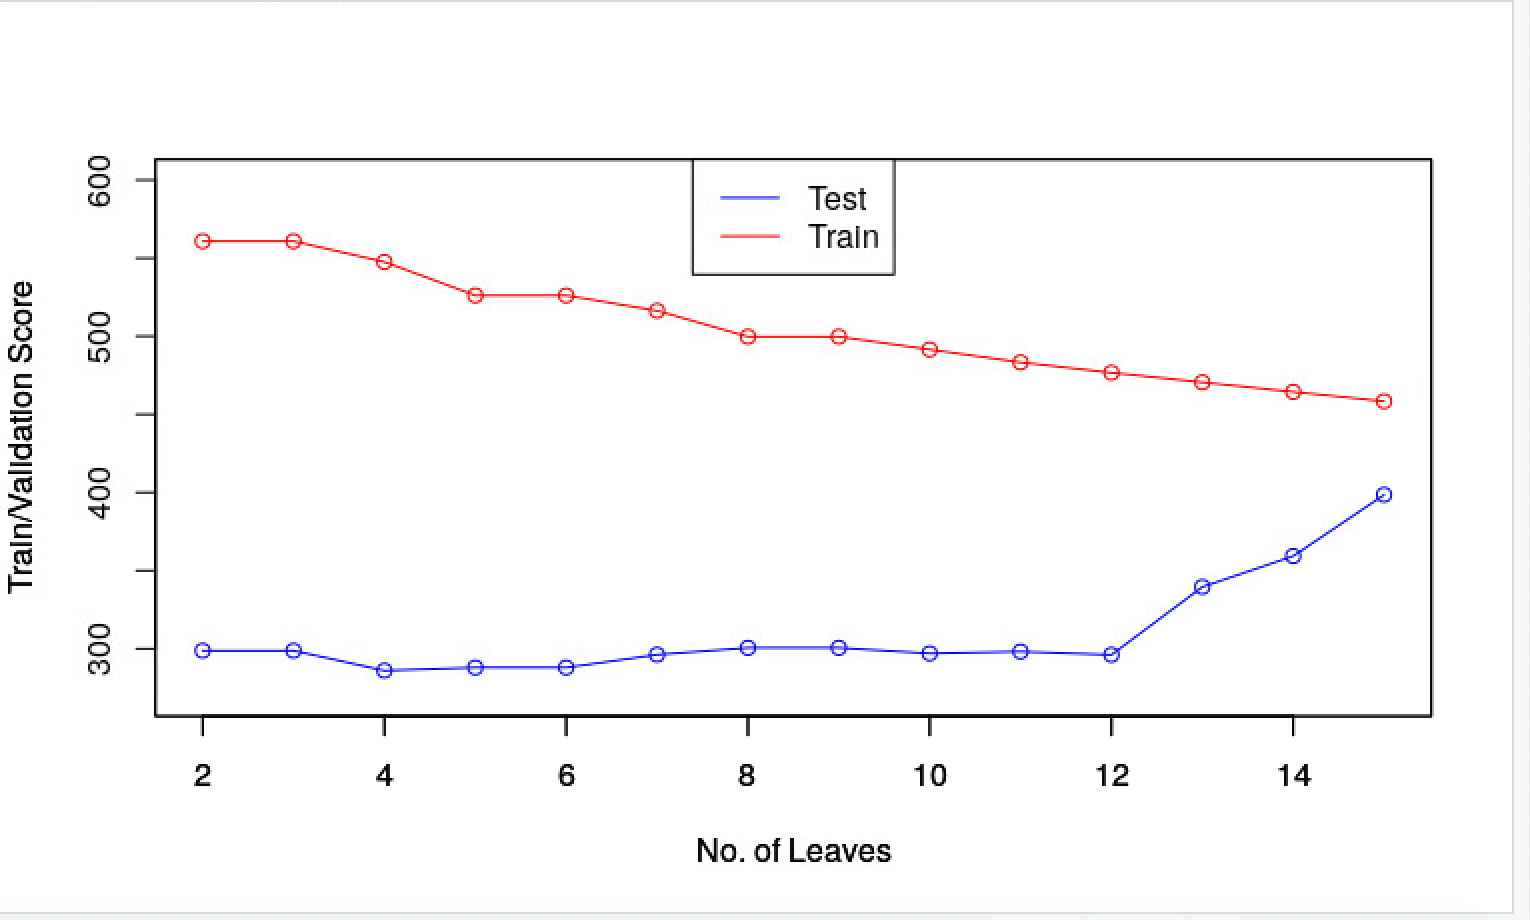
\includegraphics[width=125mm,scale=0.10]{Deviance_Dependance_train_validation_plot.png} 
\end{center} \newpage
From the above plot, I can see that deviance is low when the number of leaves are \textbf{4} with misclassification rate = \textbf{0.256} and below is the optimal tree \par
\begin{center}
  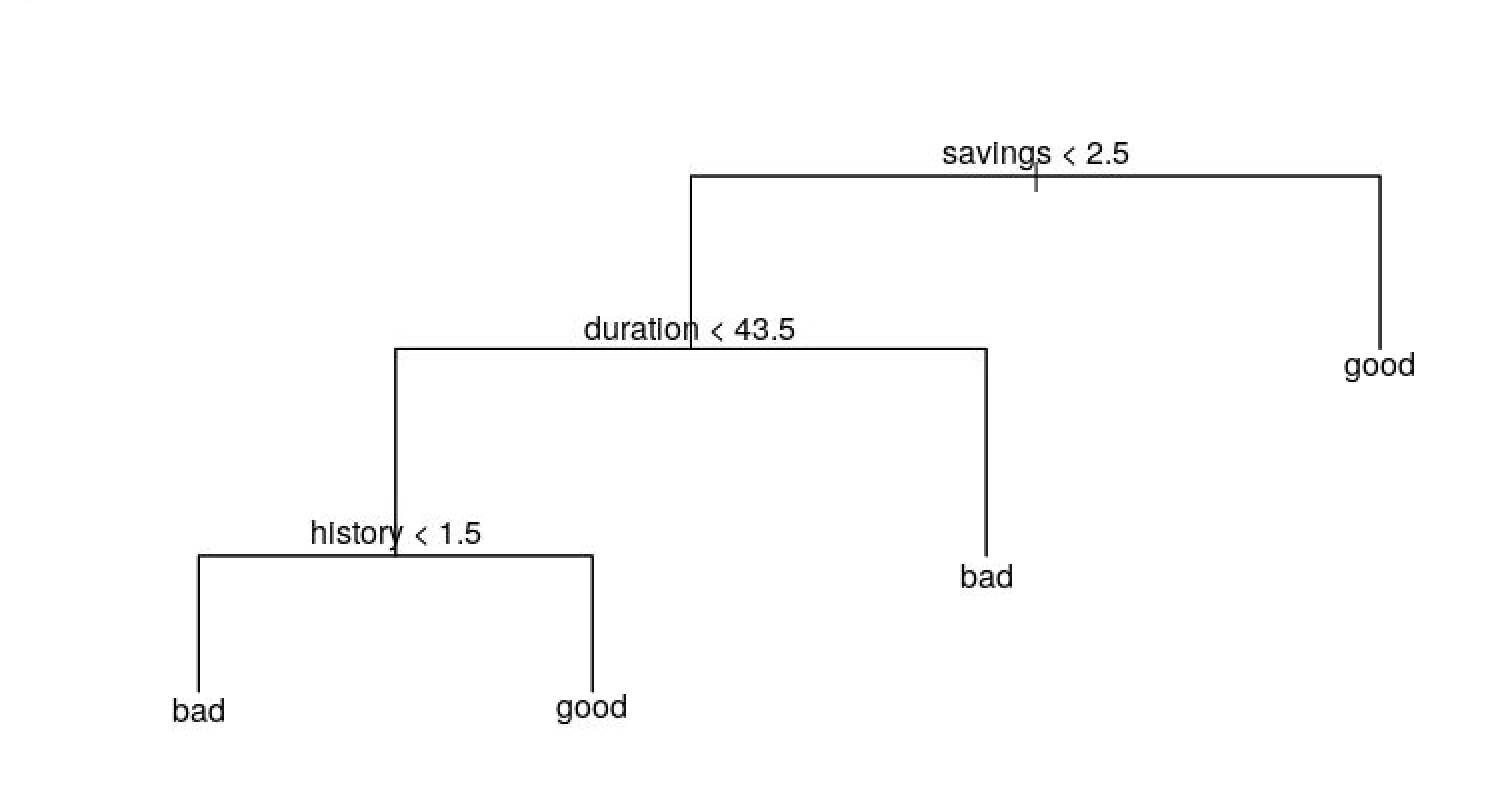
\includegraphics[width=125mm,scale=0.10]{Optimal_Tree_After_Pruning.png} 
\end{center} \par
\vspace{0.5cm}
4. I have performed Naive Bayes classification on train and test data, corresponding confusion matrix as well as misclassification rates are given below \par
\begin{center}
  \begin{tabular}{|c|c|}
    \hline
    \textbf{Confuion Matrix Train} & \textbf{Confusion Matrix Test} \\
    \hline
    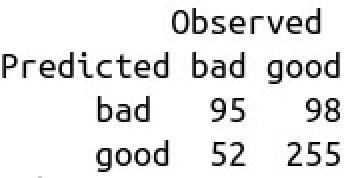
\includegraphics[width=50mm,scale=0.10]{Naive_Bayes_Train_CM.png} & 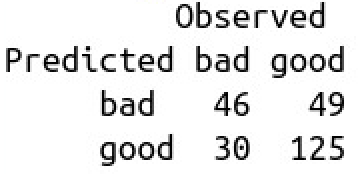
\includegraphics[width=50mm,scale=0.10]{Naive_Bayes_Test_CM.png} \\
    \hline
  \end{tabular} \par
  \begin{tabular}{|c|c|}
    \hline
    \textbf{Misclassification Rate Train} & \textbf{Misclassification Rate Test} \\
    \hline
    0.3 $\sim$ 30\% & 0.316 $\sim$ 31.6\% \\
    \hline
  \end{tabular}
\end{center}
From the above misclassification rates as well as confusion matrix, I could see that decision tree in question 2 works better for this data. \par
\vspace{0.5cm}
5. Using $\pi$ value in the range of 0.05 to 0.95, I have calculated TPR and FPR for optimal tree and naive bayes model and ROC plot is given below \par
\begin{center}
  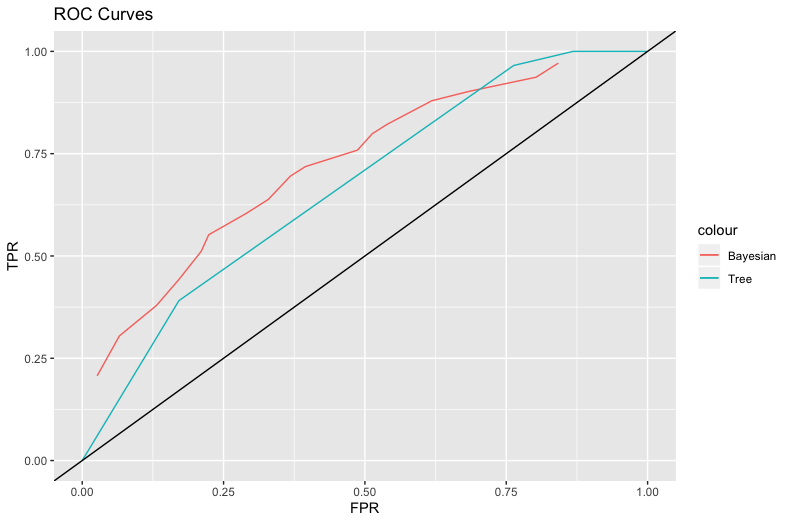
\includegraphics[width=125mm,scale=0.10]{ROC_AUC_Curve.png} 
\end{center}
From the above, ROC plot, I can say that naive bayes model performs better when compared with tree model because bayesian model has larger area under its curve.
\par
\vspace{0.5cm}
6. I have repeated the same naive bayes classification with a loss matrix and found the below Missclassification rates and Confuion matrices.\par
\begin{center}
  \begin{tabular}{|c|c|}
    \hline
    \textbf{Missclassification Rate Train} & \textbf{Missclassification Rate Test}\\
    \hline
    0.546 $\sim$ 54.6\% & 0.508 $\sim$ 50.8\%\\
    \hline
  \end{tabular}
  \par
  \begin{tabular}{|c|c|}
    \hline
    \textbf{Confusion Matrix Train} & \textbf{Confusion Matrix Test}\\
    \hline
    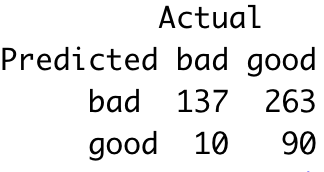
\includegraphics[width=50mm,scale=0.10]{Bayes_Loss_Matrix_Train_CM.png} & 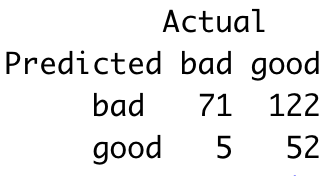
\includegraphics[width=50mm,scale=0.10]{Bayes_Loss_Matrix_Test_CM.png} \\
    \hline
  \end{tabular}
\end{center} \par
Using the loss matrix, the false positives decreased but we are predicting way more false negatives, it is because we are penalizing the false positives 10 times more than the false negatives.
In the end, the misclassification rate is way higher than when did not used to penalize the results differently. This could a good model in credit scoring 
perspective, where banks don't want to provide loans to people who cannot payback. 
\newpage
\textbf{\underline{Assignment - 4}} \par
\hl{Below given plots were all changed, as we removed the response variable from computations} \par
1. I have performed PCA on NIRSpectra data and got the following plots representing principal components, \par
\begin{center}
  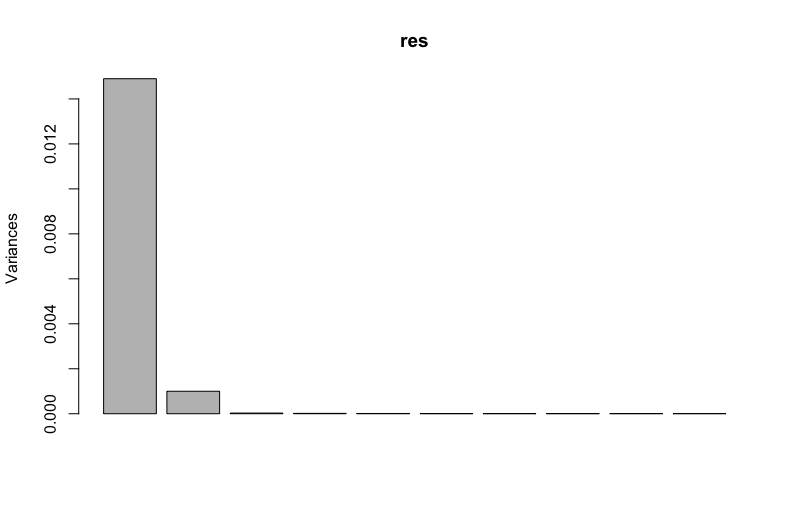
\includegraphics[width=125mm,scale=0.10]{PCA_Variance_Plot.png} 
\end{center}
The above plot tells us that, I only need 2 principal components to capture 99\% of all variance.
From the summary of \textbf{\textit{prcomp()}},
minimal number of components explaining at least 99\% of total variance are \textbf{PC1} and \textbf{PC2}. Below is the 
score plot for \textbf{PC1} and \textbf{PC2}
\begin{center}
  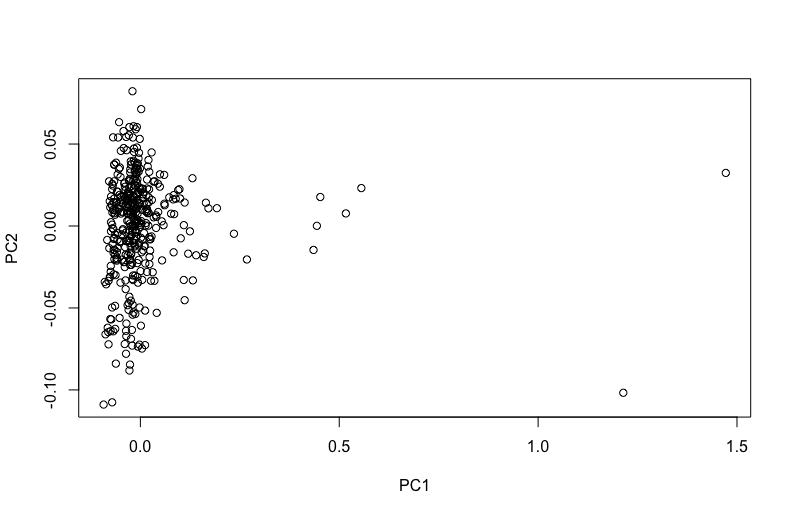
\includegraphics[width=125mm,scale=0.10]{PC1_PC2_Plot.png} 
\end{center}
Yes, from the above plot I can see there are some unusual diesel fuels above \par
2. The trace plot PC1 and PC2 are given below, \par
\begin{center}
    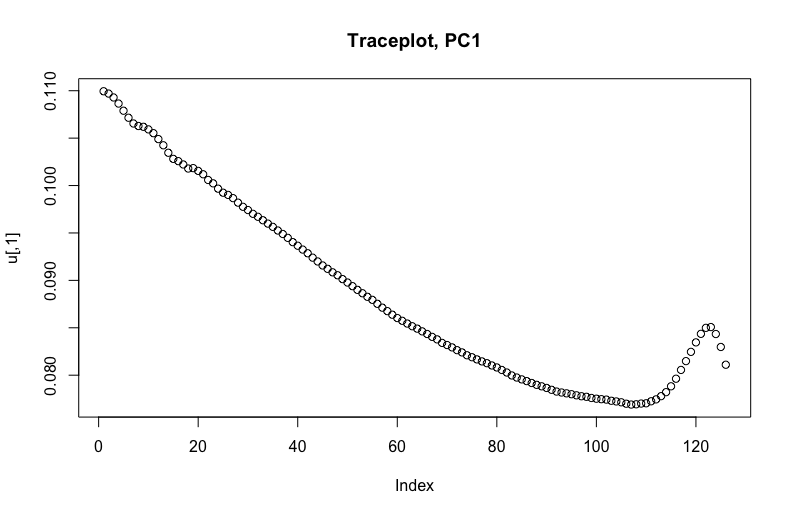
\includegraphics[width=125mm,scale=0.10]{Traceplot_PC1.png} \par
    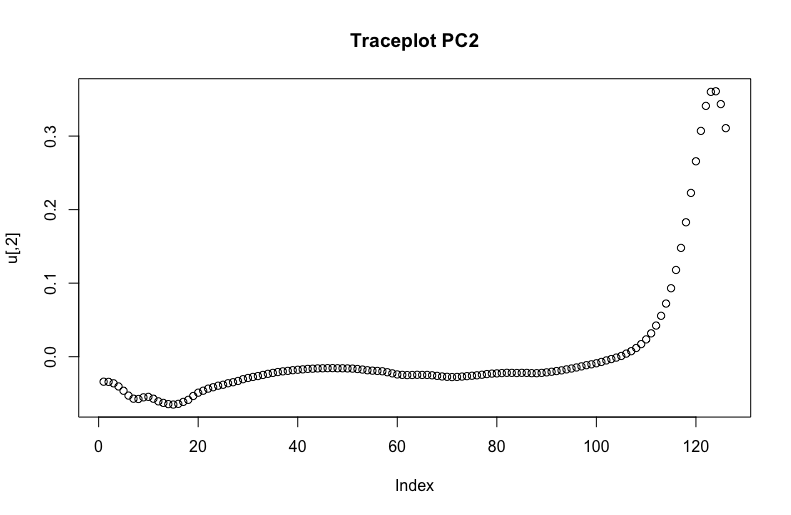
\includegraphics[width=125mm,scale=0.10]{Traceplot_PC2.png}
\end{center} \par
Performing rotation, makes the values of correlated variables into set of uncorrelated variables known as principal components.
From the trace plots of PC1 and PC2, I could see that in both PC1 and PC2 are described by most of the features, but PC1 has a feature around 120 that explains most of it. \par
\newpage
3. a. From the below plots we can see that, ICA has reversed PC2 when compared with traceplots from question 2. W' represents un-mixing (separating data into independent components) matrix
projected onto principal components. \par
\begin{center}
  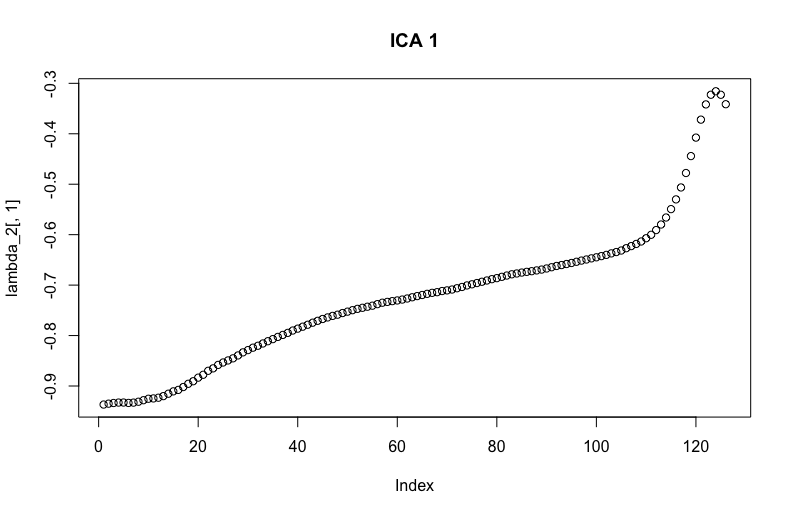
\includegraphics[width=125mm,scale=0.10]{Latent_Features_1_Traceplot.png} \par
  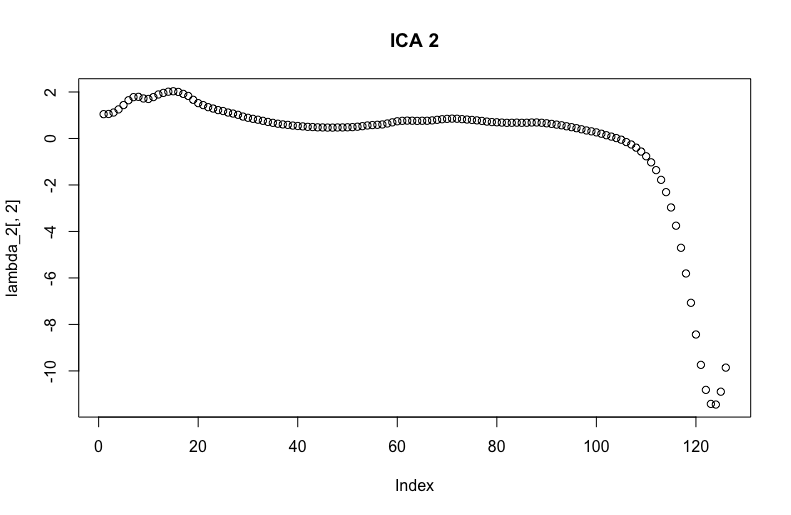
\includegraphics[width=125mm,scale=0.10]{Latent_Features_2_Traceplot.png}
\end{center} \par
\newpage
b. When comparing the below latent features plot with the plot from question 2, they look exactly same except they are reversed.
\begin{center}
  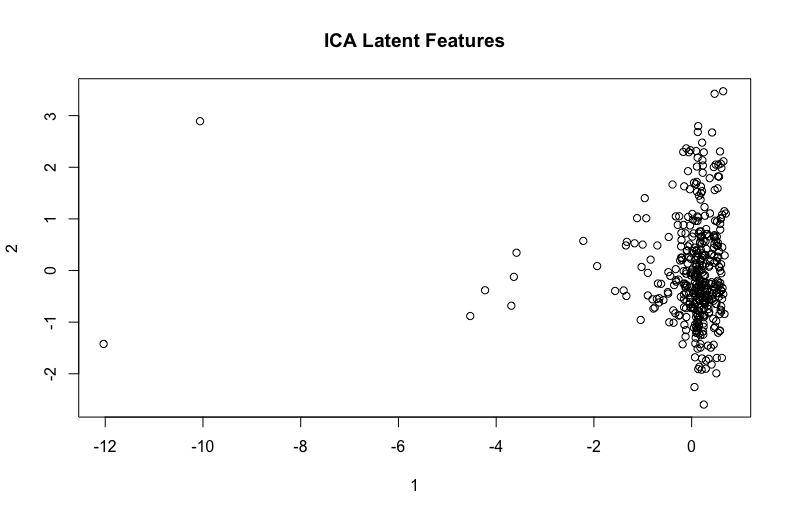
\includegraphics[width=125mm,scale=0.10]{Scoreplot_Latent_Features_ICA.png}
\end{center}
\par
\vspace{0.5cm}
\hl{We forgot to append the source code in the group report and appended it now in the group report} \par
\huge \textbf{\emph{\underline{Code Appendix}}} \par
\large \textit{\textbf{Assignment 1}} \par
\begin{lstlisting}
library(ggplot2) #Library to visualize data
library(MASS) #Library for lda()
options(scipen=999) #To avoid scientific notations
set.seed(12345)
RNGversion('3.5.1')
#Loading the data
australianCrabs = read.csv("australian-crabs.csv",stringsAsFactors = FALSE)

#Function to calculate misclassification rate
missclass=function(actualData,predictedData){
  n=length(actualData)
  return(1-sum(diag(table(actualData,predictedData)))/n)
}

#1. 
ggplot(australianCrabs,aes(x=CL,y=RW,colour=sex,shape=sex))+geom_point()

#2. Performing LDA
ldaFit = lda(sex~CL+RW,data = australianCrabs[,-c(3)],prior=c(0.5,0.5))
ldaFit
ldaFit.values = predict(ldaFit,type="response")
newData_1 = data.frame(CL=australianCrabs[,6],RW=australianCrabs[,5],
      PredictedSex=ldaFit.values$class)
ggplot(newData_1)+
  geom_point(aes(CL,RW,colour=PredictedSex),size=2.5)

table("predicted_value"=as.factor(newData_1$PredictedSex),as.factor(australianCrabs$sex))
missclass(as.factor(australianCrabs$sex),as.factor(newData_1$PredictedSex))

#3. Performing LDA with different priors
ldaFit_2 = lda(sex~CL+RW,data = australianCrabs[,-c(3)],prior=c(0.1,0.9))
ldaFit_2
ldaFit_2.values = predict(ldaFit_2,type="response")
newData_2 = data.frame(CL=australianCrabs[,6],RW=australianCrabs[,5],
      PredictedSex=ldaFit_2.values$class)
ggplot(newData_2)+
  geom_point(aes(CL,RW,colour=PredictedSex),size=2.5)

table("Predicted" = as.factor(newData_2$PredictedSex),"Actual"=australianCrabs$sex)
missclass(australianCrabs$sex,newData_2$PredictedSex)

#4. Logistic Regression
australianCrabs['Sex'] = as.factor(ifelse(australianCrabs$sex=="Male",1,0))
logisticReg = glm(Sex~CL+RW,data = australianCrabs[,-c(3)],family = "binomial")
summary(logisticReg)
logisticReg_Predict = predict(logisticReg,australianCrabs,type="response")
logisticReg_Predict_Final = ifelse(logisticReg_Predict>0.5,"Male","Female")
table("Predicted"=as.factor(logisticReg_Predict_Final),
          "Actual"=ifelse(australianCrabs$Sex==1,"Male","Female"))
missclass(australianCrabs$Sex,as.factor(logisticReg_Predict_Final))

ggplot(australianCrabs)+
  geom_point(aes(CL,RW,colour=logisticReg_Predict_Final),size=2.5)+
  geom_abline(slope = coef(logisticReg)[2]/(-coef(logisticReg)[3]) ,intercept = coef(logisticReg)[1]/(-coef(logisticReg)[3]),col="red")

\end{lstlisting}
\par
\vspace{0.5cm}
\large \textit{\textbf{Assignment 2}} \par
\begin{lstlisting}
library(ggplot2) #Library to visualize data
options(scipen=999) #To avoid scientific notations
#set.seed(12345)
RNGversion('3.5.1')
library(readxl)
library(e1071)
library(tree)
library(MASS)
library(e1071)

#Loading Data
creditScoring = read_excel("creditscoring.xls")

#Function to calculate misclassification rate
missclass=function(actualData,predictedData){
  n=length(actualData)
  return(1-sum(diag(table(actualData,predictedData)))/n)
}

creditScoring$good_bad = as.factor(creditScoring$good_bad)
n = dim(creditScoring)[1]
set.seed(12345)
id = sample(1:n,floor(n*0.5))
train = creditScoring[id,]

id1 = setdiff(1:n,id)
set.seed(12345)
id2 = sample(id1,floor(n*0.25))
valid = creditScoring[id2,]

id3 = setdiff(id1,id2)
test = creditScoring[id3,]

#2. Decision tree - measure of impurity
  #Deviance
deviance_Tree = tree(good_bad~.,data = train,split = c("deviance"))

deviance_Predicted_Test = predict(deviance_Tree,newdata=test,type="class")
missclass(as.factor(test$good_bad),deviance_Predicted_Test)

deviance_Predicted_Train = predict(deviance_Tree,newdata = train,type="class")
missclass(as.factor(train$good_bad),deviance_Predicted_Train)

  #gini
gini_Tree = tree(good_bad~.,data = train,split = c("gini"))

gini_Predicted_Test = predict(gini_Tree,newdata = test,type="class")
missclass(test$good_bad,gini_Predicted_Test)

gini_Predicted_Train = predict(gini_Tree,newdata=train,type="class")
missclass(train$good_bad,gini_Predicted_Train)

summary(deviance_Tree)
summary(gini_Tree)

#3 Choose optimal tree depth
tree_1 = tree(good_bad~.,data = train,split = c("deviance"))
summary(tree_1)
terminalNodes = 15
trainScore = rep(0,terminalNodes)
validationScore = rep(0,terminalNodes)
missclassification_Rate = c()
for(i in 2:terminalNodes){
  tree_1_Prune = prune.tree(tree_1,best=i)
  print(i)
  pred = predict(tree_1_Prune,newdata = valid,type="tree")
  trainScore[i] = deviance(tree_1_Prune)
  validationScore[i] = deviance(pred)
}

plot(2:terminalNodes,trainScore[2:terminalNodes],type="l",ylim=c(270,600),col="red",pch = "o",ylab = "Train/Test Score",xlab="No. of Leaves")
points(2:terminalNodes,trainScore[2:terminalNodes],col="red")
par(new = TRUE)
plot(2:terminalNodes,validationScore[2:terminalNodes],type="l",
          ylim=c(270,600),col="blue",pch = "o",ylab = "Train/Test Score",yaxt="n",xlab="No. of Leaves")
points(2:terminalNodes,validationScore[2:terminalNodes],col="blue")
legend(x="top",legend = c("Test","Train"),lwd=1,col=c("Blue","Red"),lty=1)

final_Pruned_Tree = prune.tree(tree_1,best = 4)
summary(final_Pruned_Tree)
plot(final_Pruned_Tree)
text(final_Pruned_Tree,pretty = 0)

pred_train_using_pruned_tree = stats::predict(final_Pruned_Tree,train,type="class")
table(pred_train_using_pruned_tree,train$good_bad)
missclass(train$good_bad,pred_train_using_pruned_tree)

pred_test_using_pruned_tree = stats::predict(final_Pruned_Tree,test,type="class")
table(pred_test_using_pruned_tree,test$good_bad)
missclass(test$good_bad,pred_test_using_pruned_tree)

#4. Naive Bayes
naive_Bayes_Fit = naiveBayes(good_bad~.,data = train)
naive_Bayes_Fit

y_train_pred_naive_bayes = stats::predict(naive_Bayes_Fit,train)
table(y_train_pred_naive_bayes,train$good_bad)
missclass(train$good_bad,y_train_pred_naive_bayes)

y_pred_naive_bayes = stats::predict(naive_Bayes_Fit,test)
table(y_pred_naive_bayes,test$good_bad)
missclass(test$good_bad,y_pred_naive_bayes)

#5.
library(caret)
pi = seq(from=0.05,to=0.95,by=0.05)
#1. optimal tree
optimal_tree_vector = stats::predict(final_Pruned_Tree,test,type="vector")
naive_Bayes_raw = stats::predict(naive_Bayes_Fit,test,type="raw")
tree_tpr = c()
tree_fpr = c()
bayes_tpr = c()
bayes_fpr = c()
for(i in 1:length(pi))
{
  temp1 = confusionMatrix(as.factor(ifelse(optimal_tree_vector[,2]>pi[i],"good","bad")),
                          test$good_bad)
  tree_tpr[i] = temp1$table[4]/(temp1$table[4]+temp1$table[3])
  tree_fpr[i] = temp1$table[2]/(temp1$table[2]+temp1$table[1])
  temp2 = confusionMatrix(as.factor(ifelse(naive_Bayes_raw[,2]>pi[i],"good","bad")),
                          test$good_bad)
  bayes_tpr[i] = temp2$table[4]/(temp2$table[4]+temp2$table[3])
  bayes_fpr[i] = temp2$table[2]/(temp2$table[2]+temp2$table[1])
}

roc_Df = data.frame(tree_tpr = tree_tpr,tree_fpr = tree_fpr,bayes_tpr=bayes_tpr,bayes_fpr = bayes_fpr)

ggplot(roc_Df) + geom_line(aes(x=bayes_fpr, y = bayes_tpr, color = 'Bayesian')) + geom_line(aes(x=tree_fpr, y = tree_tpr, color = 'Tree')) +
geom_abline(slope=1,intercept = 0)+ ggtitle("ROC Curves")+xlab("FPR")+ylab("TPR")

#6.
prob_Naive_Bayes_test = predict(naive_Bayes_Fit,newdata = test,type = c("raw"))
weighted_Naive_Bayes_Pred_Test_Data = replace(prob_Naive_Bayes_test,
          prob_Naive_Bayes_test[,1]*10>prob_Naive_Bayes_test[,2],"bad")
weighted_Naive_Bayes_Pred_Test_Data = replace(weighted_Naive_Bayes_Pred_Test_Data,
          prob_Naive_Bayes_test[,1]*10<=prob_Naive_Bayes_test[,2],"good")
table("Predicted"=as.factor(weighted_Naive_Bayes_Pred_Test_Data[,1]),
          "Actual"=test$good_bad)
missclass(test$good_bad,as.factor(weighted_Naive_Bayes_Pred_Test_Data[,1]))

prob_Naive_Bayes_train = predict(naive_Bayes_Fit,newdata = train,type = c("raw"))
weighted_Naive_Bayes_Pred_Train_Data = replace(prob_Naive_Bayes_train,
          prob_Naive_Bayes_train[,1]*10>prob_Naive_Bayes_train[,2],"bad")
weighted_Naive_Bayes_Pred_Train_Data = replace(weighted_Naive_Bayes_Pred_Train_Data,
          prob_Naive_Bayes_train[,1]*10<=prob_Naive_Bayes_train[,2],"good")
table("Predicted"=as.factor(weighted_Naive_Bayes_Pred_Train_Data[,1]),
         "Actual"=train$good_bad)
missclass(train$good_bad,as.factor(weighted_Naive_Bayes_Pred_Train_Data[,1]))
\end{lstlisting}
\par
\vspace{0.5cm}
\large \textit{\textbf{Assignment 4}} \par
\begin{lstlisting}
  options(scipen=999) #To avoid scientific notations
  set.seed(12345)
  RNGversion('3.5.1')
  nirSpectra = read.csv2("NIRspectra.csv",stringsAsFactors = FALSE)
  
  #1. Applying PCA
  drops = c("Viscosity")
  nirSpectra = nirSpectra[,!(names(nirSpectra) %in% drops)]
  nirSpectra$Viscosity = c()
  res = prcomp(nirSpectra)
  lambda = res$sdev^2
  sprintf("%2.3f",lambda/sum(lambda)*100)
  screeplot(res)
  
  plot(res$x[,1],res$x[,2],xlab = "PC1",ylab = "PC2")
  
  #2. Traceplots
  u = res$rotation
  plot(u[,1],main="Traceplot, PC1",ylab = "u[,1]")
  plot(u[,2],main="Traceplot PC2",ylab = "u[,2]")
  
  #3. fastICA
  set.seed(12345)
  ica = fastICA::fastICA(nirSpectra,2)
  lambda_2 = ica$K%*%ica$W
  plot(lambda_2[,1],main="ICA 1")
  plot(lambda_2[,2],main="ICA 2")
  
  plot(ica$S[,1],ica$S[,2],main="ICA Latent Features",xlab="1",ylab="2")  
\end{lstlisting}
\end{document}